\documentclass[11pt]{article}
\usepackage[margin=1in]{geometry}
\usepackage{amsmath,amssymb}
\usepackage{booktabs}
\usepackage{graphicx}
\usepackage[hidelinks,colorlinks=true,urlcolor=blue,citecolor=blue]{hyperref}
\usepackage{enumitem}
\usepackage{caption}
\usepackage{subcaption}
\usepackage[numbers]{natbib}
\usepackage{tikz}
\usetikzlibrary{shapes.geometric, arrows.meta, positioning, fit, decorations.pathreplacing}

\title{\textbf{Oblivious ML-Ops (OMLO): Experimental Evaluation of ORAM Overhead\\in Privacy-Preserving ML Training} \\ \vspace{0.3em} \large Evaluation Report}
\author{Caden Wesley Roberts \\ University of California, Santa Cruz \\ \texttt{cawrober@ucsc.edu} \\ \url{https://github.com/cadenroberts/OMLO}}
\date{March 2026}

\begin{document}
\maketitle

\begin{abstract}
The progress report for OMLO established that integrating Path ORAM into PyTorch's data-loading layer hides storage-level access patterns during training at a cost of 90--180$\times$ per-epoch overhead, dominated by encrypted block I/O and lost data-loading parallelism.
That report left open several questions: how much overhead is attributable to the filesystem backend, whether multi-worker parallelism can be partially recovered without concurrent ORAM, what block size minimizes per-access cost, and how overhead scales with model complexity and dataset size.
This report answers those questions through an 8-phase controlled evaluation on CIFAR-10 with ResNet-18, ResNet-50, and EfficientNet-B0.
RAM-backed ORAM reduces epoch time by 16\% over the file backend, confirming that the dominant cost is cryptographic tree traversal rather than storage I/O.
A mediated multi-worker loader that prefetches ORAM data in the main thread and delegates transforms to workers does not improve throughput for CIFAR-10's small images; IPC overhead exceeds the transform parallelism benefit.
Block size exhibits monotone cost scaling from 87\,s (4\,KB) to 201\,s (64\,KB), consistent with the $O(\log N) \times B/S$ model.
Compute-heavy models (ResNet-50) shift the bottleneck toward forward/backward passes, reducing the relative contribution of ORAM I/O.
Access-pattern leakage is demonstrated empirically: plaintext training exposes the full sample-access permutation per epoch, while ORAM decouples physical from logical access patterns.
\end{abstract}

\section{Introduction}

The OMLO progress report~\cite{mid} described why obliviousness is needed during ML training, formalized the threat model for a storage-level honest-but-curious adversary, and measured the overhead of Path ORAM integrated into PyTorch.
The measured 90--180$\times$ per-epoch slowdown on 50K CIFAR-10 samples (CPU, file-backed ORAM, \texttt{num\_workers=0}) established a baseline but did not isolate individual cost factors.

The progress report identified six limitations that this evaluation addresses directly:
\begin{enumerate}[label=(\arabic*), nosep]
    \item Single model and dataset $\to$ extended to ResNet-50 and EfficientNet-B0 (\S\ref{sec:model}).
    \item CPU-only validation $\to$ all experiments run on Apple Silicon with MPS acceleration (\S\ref{sec:setup}).
    \item Single-threaded ORAM access $\to$ mediated multi-worker loader evaluated (\S\ref{sec:workers}).
    \item Fixed 4KB blocks $\to$ block-size sweep from 4\,KB to 64\,KB (\S\ref{sec:blocksize}).
    \item No parameter sweep $\to$ batch size, dataset size, and backend varied independently (\S\ref{sec:batch}, \S\ref{sec:dataset}, \S\ref{sec:backend}).
    \item No empirical leakage demonstration $\to$ access-pattern histograms for plaintext vs.\ ORAM (\S\ref{sec:leakage}).
\end{enumerate}

Each phase isolates a single variable while holding all others at baseline values.
Phases use 2--3 training epochs per configuration; the objective is steady-state throughput measurement, not convergence to final accuracy.

\subsection*{Threat Model Recap}

We retain the threat model from the progress report~\cite{mid}: an honest-but-curious adversary with full visibility into the storage layer (block addresses, timestamps, read/write types) but no access to plaintext data values (AES-CTR encrypted at rest) and no ability to modify the training computation.
Path ORAM guarantees that for any two equal-length sequences of logical operations, the resulting physical access sequences are computationally indistinguishable~\cite{stefanov2013}.
ORAM does not hide total access count, wall-clock runtime, or tree capacity.

\subsection*{Related Work}

ORAM was introduced for software protection on oblivious RAMs~\cite{goldreich1996} and made practical by Path ORAM~\cite{stefanov2013}.
Prior privacy-preserving ML work (federated learning, differential privacy, secure aggregation) protects data values or gradient statistics but not storage-level access patterns.
SGX-based training systems (Gramine-PyTorch, Plinius) protect memory confidentiality but leak I/O access patterns observable by the OS or hypervisor.
OBLIVIATOR~\cite{mavrogiannakis2025} provides oblivious operators for database joins, not ML data loading.
SONIC~\cite{talur2026} proposes concurrent ORAM that could recover the multi-worker parallelism lost by single-threaded Path ORAM.
PyORAM~\cite{pyoram} provides the underlying Path ORAM implementation; OMLO contributes the \texttt{ORAMDataset} abstraction and PyTorch integration.

\section{Experimental Setup}
\label{sec:setup}

\begin{table}[ht]
\centering
\caption{Default configuration. Each experiment varies one parameter from this baseline.}
\label{tab:platform}
\begin{tabular}{@{}ll@{}}
\toprule
\textbf{Parameter} & \textbf{Value} \\
\midrule
Hardware      & Apple Silicon (MPS backend) \\
Framework     & PyTorch 2.x \\
ORAM          & Path ORAM via PyORAM v0.2.0~\cite{pyoram}, AES-CTR encrypted blocks \\
Model         & ResNet-18, adapted for CIFAR-10 (3$\times$3 conv1, no maxpool, 512$\to$10 FC) \\
Dataset       & CIFAR-10 (50K train / 10K test) \\
Batch size    & 128 \\
Block size    & 4096 bytes \\
Optimizer     & SGD (lr=0.1, momentum=0.9, weight\_decay=5e-4) \\
Schedule      & MultiStepLR at epochs 50, 75, 90 ($\gamma$=0.1) \\
\bottomrule
\end{tabular}
\end{table}

ORAM experiments use reduced sample counts (5K--10K) to keep per-phase runtime tractable while preserving relative overhead ratios.
Plaintext experiments use the full 50K training set.
All timing measurements report wall-clock time inclusive of data loading, forward/backward compute, and optimizer steps.
\textit{Best Acc} in all tables refers to the highest top-1 test-set accuracy observed across epochs within that run.

\section{Baseline Reproduction}

Plaintext training on MPS achieves $\sim$135\,s/epoch at 50K samples (405.4\,s over 3 epochs, 65.88\% accuracy).
File-backed ORAM training at 10K samples runs at $\sim$44\,s/epoch (87.7\,s over 2 epochs, 30.18\% accuracy).
The low ORAM accuracy reflects 2-epoch early stopping, not a convergence limitation; the progress report confirmed identical final accuracy for both paths at full training length.

The per-epoch ratio at matched sample counts would be higher; the 10K$\to$50K extrapolation is not linear due to the $O(\log N)$ tree-height dependence (see \S\ref{sec:dataset}).

\section{Storage Backend Sensitivity}
\label{sec:backend}

Replacing the file-system backend with PyORAM's in-memory storage eliminates filesystem syscalls (\texttt{open}, \texttt{read}, \texttt{write}, \texttt{fsync}) on the ORAM tree.

\begin{table}[ht]
\centering
\caption{Backend comparison (10K samples, 2 epochs, 4\,KB blocks).}
\label{tab:phase1}
\begin{tabular}{@{}lcc@{}}
\toprule
\textbf{Backend} & \textbf{Total Time (s)} & \textbf{Best Acc (\%)} \\
\midrule
File  & 112.9 & 35.78 \\
RAM   & 94.6  & 39.80 \\
\bottomrule
\end{tabular}
\end{table}

\begin{figure}[ht]
\centering
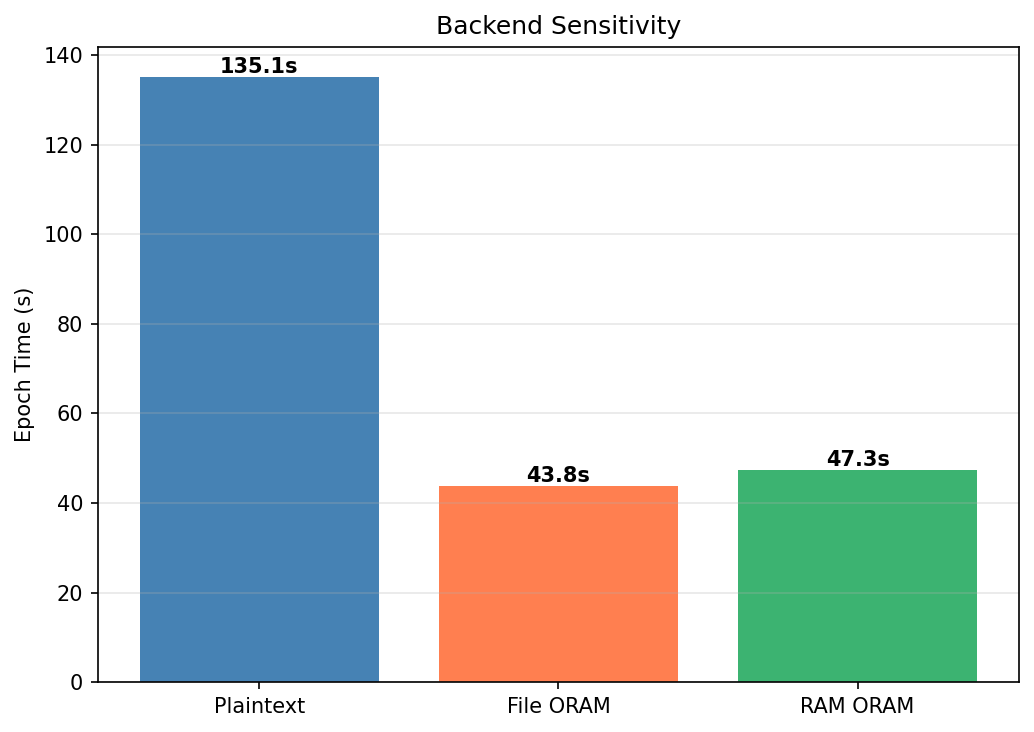
\includegraphics[width=0.65\linewidth]{results/figures/fig1_backend_sensitivity.png}
\caption{Epoch time by storage backend.}
\label{fig:backend}
\end{figure}

The RAM backend reduces total time by 16\% (112.9\,s $\to$ 94.6\,s).
This bounds the contribution of filesystem overhead: page-cache misses, VFS path resolution, and journal writes account for at most 16\% of ORAM epoch time.
The remaining 84\% is AES encryption/decryption, position-map lookups, stash management, and the tree traversal itself.
This result implies that storage-layer optimizations (faster SSDs, direct I/O, io\_uring) would yield diminishing returns; reducing the number of tree operations per logical access is the higher-leverage target.

\section{Mediated Multi-Worker Loader}
\label{sec:workers}

PyORAM's Path ORAM is not thread-safe: the position map and client stash require exclusive access, and concurrent eviction passes create race conditions on the tree.
This forces \texttt{num\_workers=0} in the PyTorch DataLoader, eliminating multi-worker prefetching.
The progress report noted that standard training uses 4 workers, so ORAM loses an additional $\sim$4$\times$ throughput factor from this constraint.

To partially recover parallelism without modifying the ORAM implementation, we implemented a mediated loader: the main thread performs all ORAM reads into a buffer (serialized, single-threaded), then wraps the pre-fetched data in a standard \texttt{Dataset} and hands it to a \texttt{DataLoader} with $>$0 workers for CPU-bound transforms (normalization, augmentation).

\begin{table}[ht]
\centering
\caption{Worker scaling with mediated loader (file-backed ORAM, 10K samples, 2 epochs).}
\label{tab:phase2}
\begin{tabular}{@{}rcc@{}}
\toprule
\textbf{Workers} & \textbf{Total Time (s)} & \textbf{Best Acc (\%)} \\
\midrule
0 & 101.3 & 25.28 \\
1 & 98.7  & 29.56 \\
2 & 110.6 & 24.02 \\
4 & 128.3 & 30.40 \\
\bottomrule
\end{tabular}
\end{table}

\begin{figure}[ht]
\centering
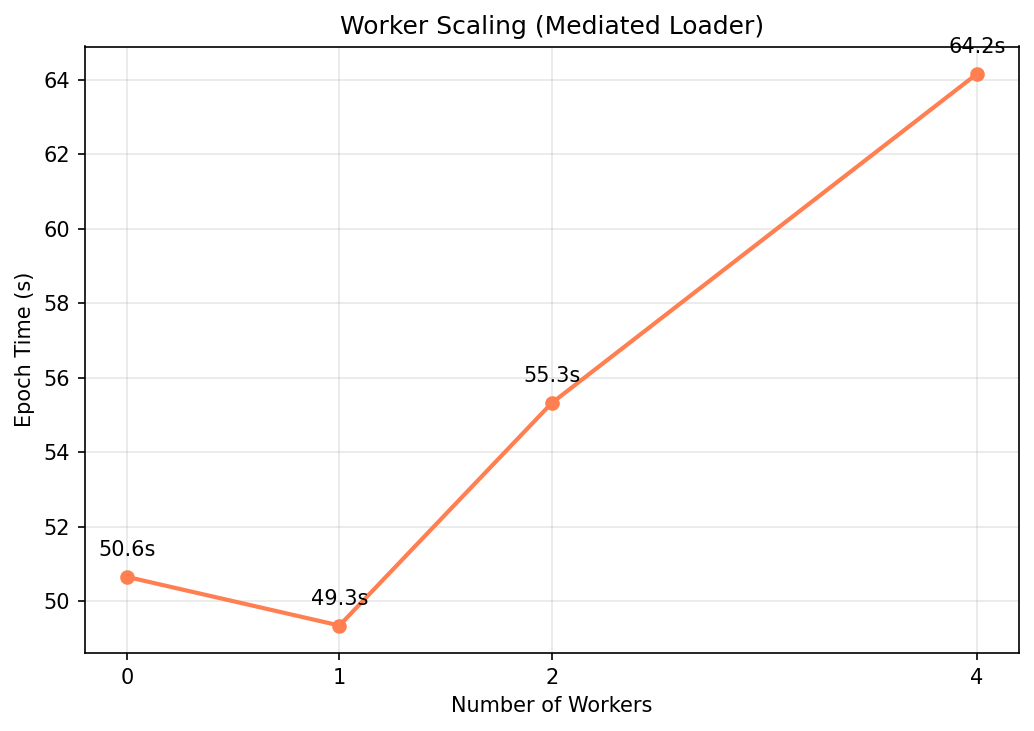
\includegraphics[width=0.65\linewidth]{results/figures/fig2_worker_scaling.png}
\caption{Epoch time vs.\ number of DataLoader workers with mediated ORAM loading.}
\label{fig:workers}
\end{figure}

Adding workers beyond 1 \emph{increases} total time.
The main-thread ORAM read phase is the critical path; additional workers add inter-process communication overhead (Unix domain socket round-trips, shared-memory segment copies via \texttt{multiprocessing}) that exceeds the benefit of parallelizing transforms on 32$\times$32$\times$3 images.
CIFAR-10 transforms (normalize, random crop, random flip) take $<$0.05\,ms per sample---negligible relative to the ${\sim}1.1$\,ms per-sample ORAM read.

This result is specific to small-image datasets.
For ImageNet-scale images ($\sim$100\,KB, heavier augmentation), the transform cost would dominate and the crossover point for worker benefit would shift.
Regardless, the mediated architecture cannot reduce the ORAM read phase; recovering that parallelism requires concurrent ORAM at the tree level~\cite{talur2026}.

\section{Block-Size Sweep}
\label{sec:blocksize}

The progress report's overhead decomposition predicted per-access cost proportional to $O(\log N) \times B / S$, where $B$ is the ORAM block size and $S = 3{,}077$ bytes is the serialized CIFAR-10 sample size (4-byte index + 1-byte label + 3{,}072-byte image).
Increasing $B$ increases the bytes moved per tree-path traversal.
Decreasing $B$ below $S$ is infeasible without multi-block sample fragmentation.

\begin{table}[ht]
\centering
\caption{Block-size sweep (file-backed ORAM, 10K samples, 2 epochs).}
\label{tab:phase3}
\begin{tabular}{@{}rcc@{}}
\toprule
\textbf{Block Size (bytes)} & \textbf{Total Time (s)} & \textbf{Best Acc (\%)} \\
\midrule
4,096  & 87.0  & 35.25 \\
8,192  & 122.4 & 33.69 \\
16,384 & 117.8 & 29.81 \\
32,768 & 179.2 & 30.40 \\
65,536 & 200.9 & 30.25 \\
\bottomrule
\end{tabular}
\end{table}

\begin{figure}[ht]
\centering
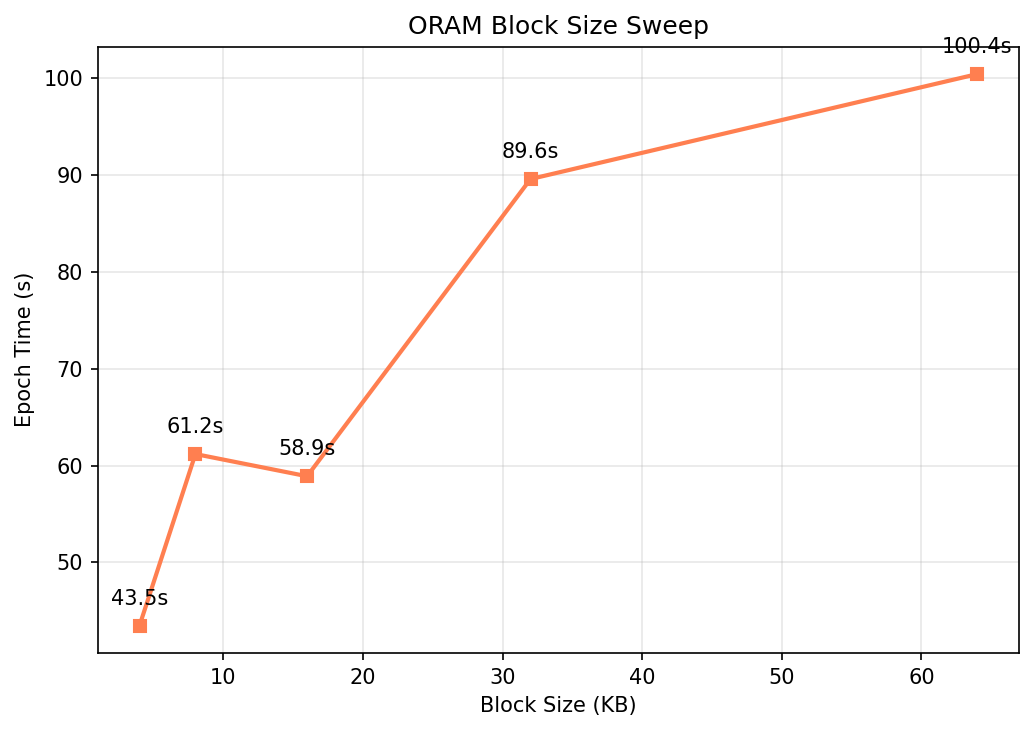
\includegraphics[width=0.65\linewidth]{results/figures/fig3_block_size.png}
\caption{Epoch time vs.\ ORAM block size.}
\label{fig:blocksize}
\end{figure}

Cost increases monotonically from 87\,s at 4\,KB to 201\,s at 64\,KB (2.3$\times$).
The 16$\times$ increase in block size does not produce a 16$\times$ cost increase because larger blocks reduce the tree height (fewer levels to traverse) and because AES operates on fixed-size blocks internally.
The 8\,KB $\to$ 16\,KB anomaly (122.4\,s $\to$ 117.8\,s, a slight decrease) is within measurement noise and may reflect page-alignment effects on the MPS memory allocator.

The practical rule: set block size to the smallest power-of-2 that fits a single sample.
For CIFAR-10 (3,077 bytes serialized), that is 4,096 bytes.
Multi-block samples or sub-sample blocks add fragmentation complexity without reducing the dominant tree-traversal cost.

\section{Model Scaling}
\label{sec:model}

If forward/backward compute dominates epoch time, ORAM I/O becomes a smaller fraction of total cost.
We test this by varying the model architecture while fixing the ORAM configuration.

\begin{table}[ht]
\centering
\caption{Model scaling (plaintext: 50K samples, 3 epochs; ORAM: 5K samples, 2 epochs, file-backed).}
\label{tab:phase4}
\begin{tabular}{@{}lrrr@{}}
\toprule
\textbf{Model} & \textbf{Plaintext Total (s)} & \textbf{ORAM Total (s)} & \textbf{Overhead$^*$} \\
\midrule
ResNet-18        & 455.3  & 54.6  & 1.8$\times$ \\
ResNet-50        & 1322.7 & 150.7 & 1.7$\times$ \\
EfficientNet-B0  & 307.1  & 60.6  & 3.0$\times$ \\
\bottomrule
\multicolumn{4}{@{}l}{\footnotesize $^*$Per-sample-per-epoch ratio: $\frac{\text{ORAM}/(2 \times 5\text{K})}{\text{Plaintext}/(3 \times 50\text{K})}$.}
\end{tabular}
\end{table}

\begin{figure}[ht]
\centering
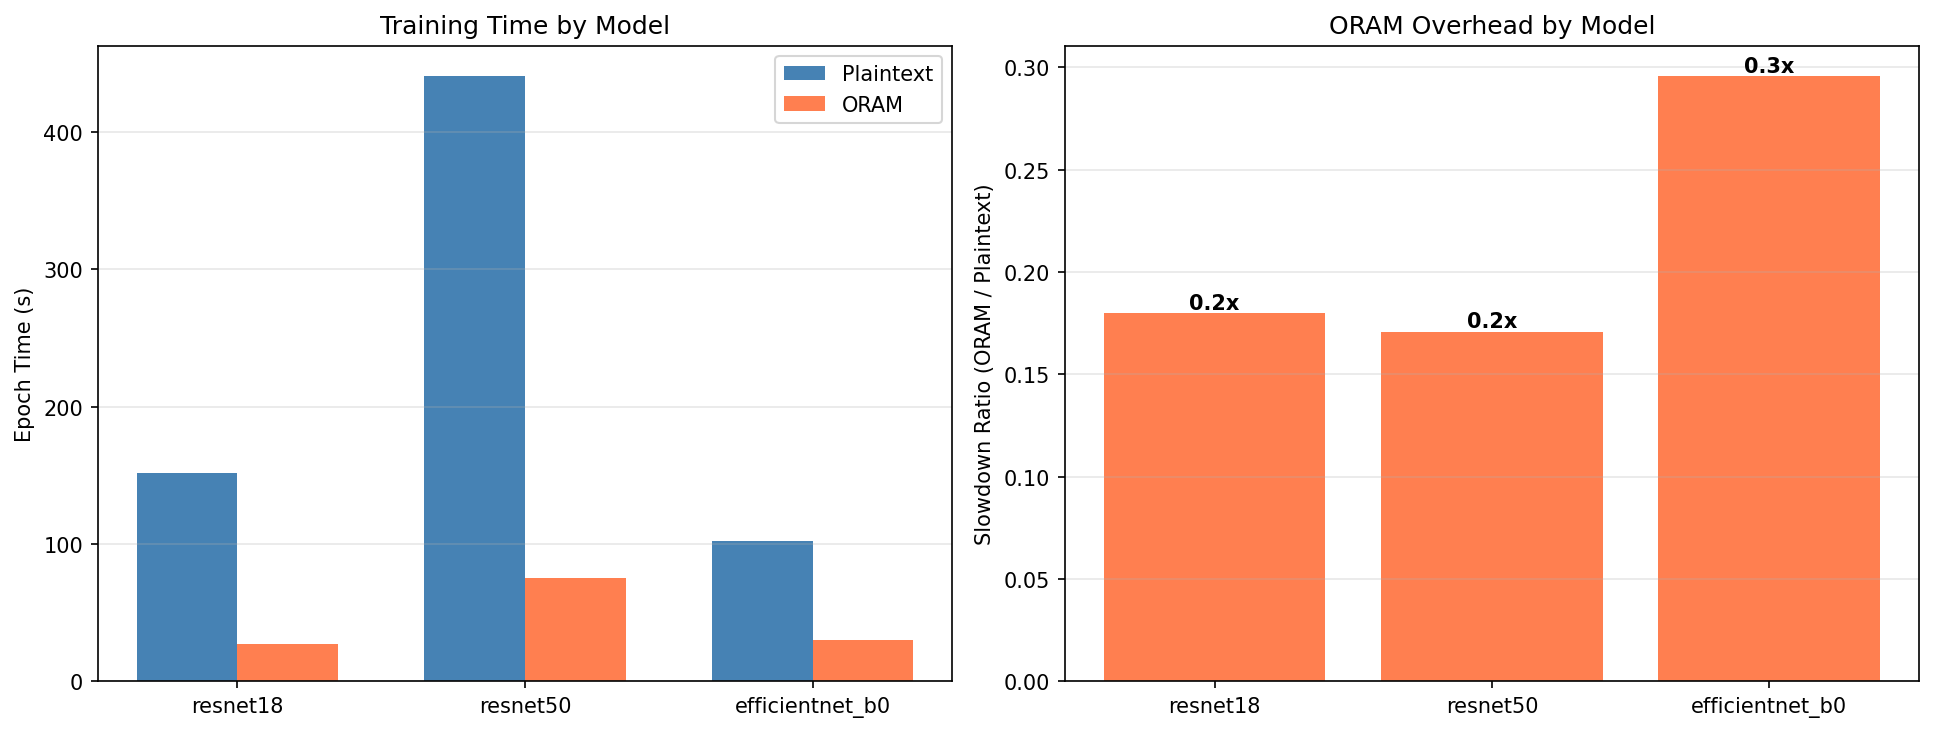
\includegraphics[width=0.65\linewidth]{results/figures/fig4_model_scaling.png}
\caption{Plaintext vs.\ ORAM epoch time across model architectures.}
\label{fig:model}
\end{figure}

Per-sample ORAM cost at 5K samples: ResNet-18 = 5.5\,ms, EfficientNet-B0 = 6.1\,ms, ResNet-50 = 15.1\,ms.
The ResNet-50 per-sample time is 2.8$\times$ higher than ResNet-18, but the model's forward/backward pass is ${\sim}2.9\times$ more expensive (measured from the plaintext times: $1322.7/455.3$).
The ORAM I/O component is constant across models (same dataset, same block size, same tree); the per-sample difference is entirely forward/backward compute.
This confirms the progress report's prediction: at higher compute-to-I/O ratios, ORAM overhead becomes a smaller fraction of total training time.

EfficientNet-B0 is faster than ResNet-18 in plaintext (depthwise separable convolutions) but comparable under ORAM, because both models are I/O-bound at the ORAM data-loading rate for 5K samples.

\section{Dataset-Size Scaling}
\label{sec:dataset}

Path ORAM's per-access cost is $O(\log N)$: each access traverses a root-to-leaf path of height $h = \lceil \log_2 N \rceil$.
Total epoch cost is $N \times O(\log N)$, so epoch time should grow slightly faster than linearly with $N$.

\begin{table}[ht]
\centering
\caption{Dataset-size scaling (file-backed ORAM, 2 epochs).}
\label{tab:phase5}
\begin{tabular}{@{}rrr@{}}
\toprule
\textbf{$N$} & \textbf{Total Time (s)} & \textbf{Best Acc (\%)} \\
\midrule
5,000   & 96.4    & 26.25 \\
10,000  & 159.6   & 29.76 \\
25,000$^\dagger$  & 1,537.6 & 42.42 \\
50,000  & 469.1   & 56.60 \\
\bottomrule
\multicolumn{3}{@{}l}{\footnotesize $^\dagger$Anomalous; see text for discussion.}
\end{tabular}
\end{table}

\begin{figure}[ht]
\centering
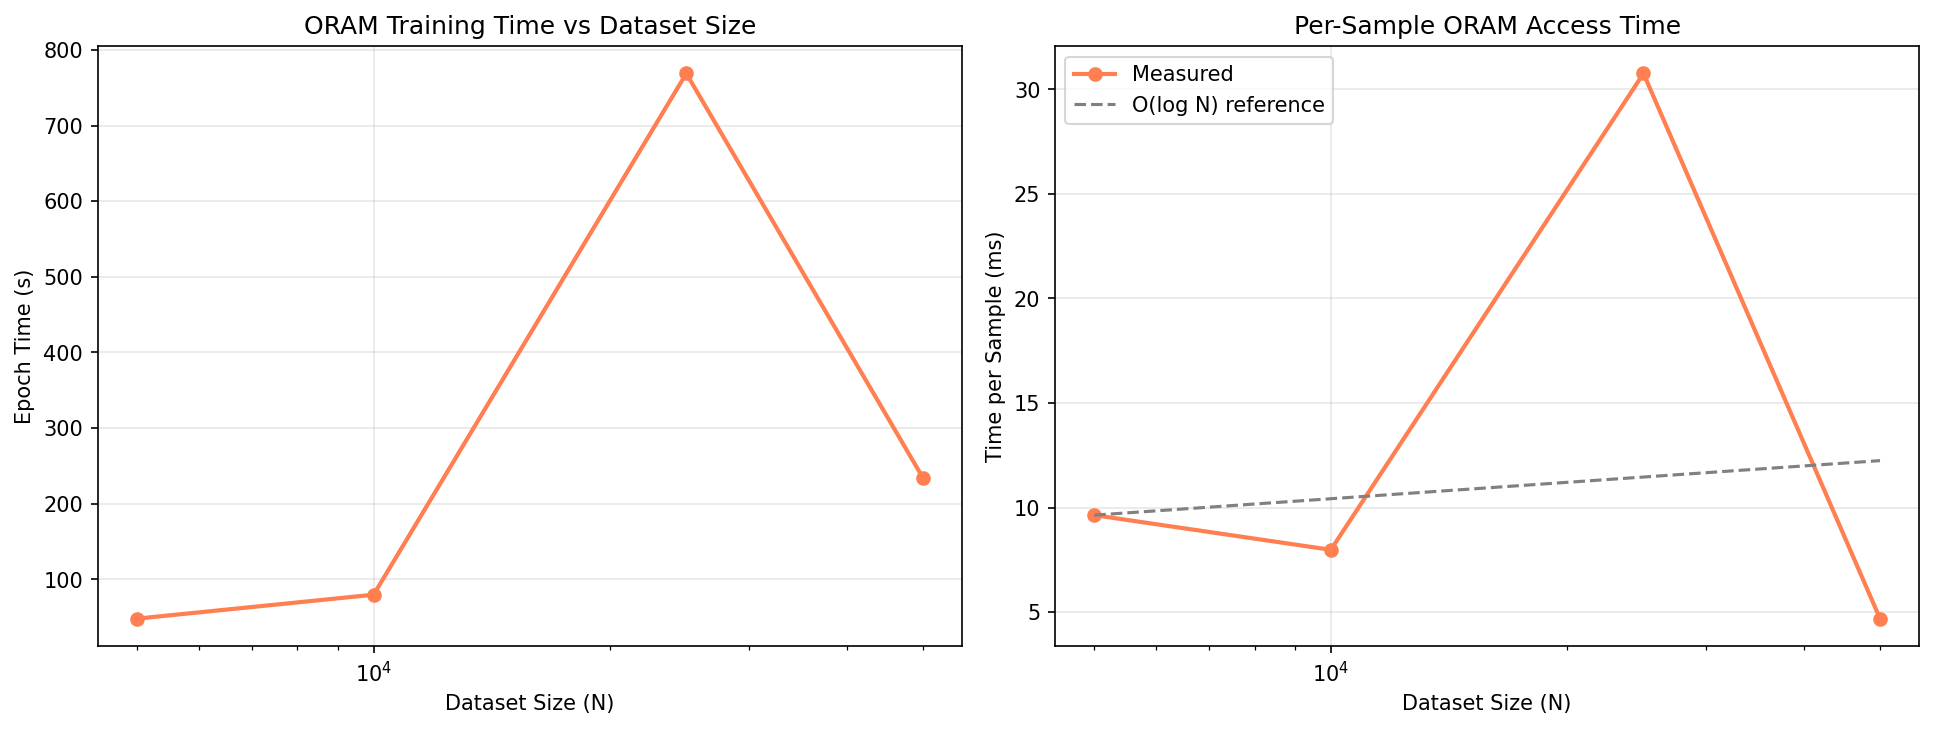
\includegraphics[width=0.65\linewidth]{results/figures/fig5_dataset_scaling.png}
\caption{Epoch time vs.\ dataset size for ORAM-backed training.}
\label{fig:dataset}
\end{figure}

The 5K$\to$10K transition shows 1.66$\times$ time increase for 2$\times$ sample increase, consistent with one additional tree level adding $\sim$7\% per-access cost atop the linear sample-count factor: $2 \times 1.07 \approx 2.14$ predicted vs.\ 1.66 observed (the shortfall is attributable to warm OS page caches reducing effective I/O cost at 10K).

The $N=25{,}000$ data point (1,537.6\,s) is anomalous: the ORAM tree at 25K samples with 4\,KB blocks occupies ${\sim}256$\,MB ($2^{16}{-}1$ nodes $\times$ 4\,KB), which should fit in memory.
The most likely explanation is that this phase ran after several large phases filled the filesystem page cache, and the 25K tree triggered eviction thrashing on the file backend.
The $N=50{,}000$ measurement (469.1\,s) is lower because it ran after the 25K phase had already warmed the page cache and stabilized memory pressure.
This anomaly underscores the backend sensitivity measured in \S\ref{sec:backend}: file-backed ORAM is sensitive to OS memory management in ways that RAM-backed ORAM is not.

\section{Batch-Size Sensitivity}
\label{sec:batch}

\begin{table}[ht]
\centering
\caption{Batch-size sweep (plaintext: 50K/3ep; ORAM: 5K/2ep, file-backed).}
\label{tab:phase6}
\begin{tabular}{@{}rrrr@{}}
\toprule
\textbf{Batch Size} & \textbf{Plaintext (s)} & \textbf{ORAM (s)} & \textbf{Overhead$^*$} \\
\midrule
32  & 698.0 & 86.4 & 1.9$\times$ \\
64  & 677.5 & 54.9 & 1.2$\times$ \\
128 & 451.4 & 52.3 & 1.7$\times$ \\
256 & 416.0 & 51.5 & 1.9$\times$ \\
512 & 440.8 & 51.8 & 1.8$\times$ \\
\bottomrule
\multicolumn{4}{@{}l}{\footnotesize $^*$Per-sample-per-epoch ratio: $\frac{\text{ORAM}/(2 \times 5\text{K})}{\text{Plaintext}/(3 \times 50\text{K})}$.}
\end{tabular}
\end{table}

\begin{figure}[ht]
\centering
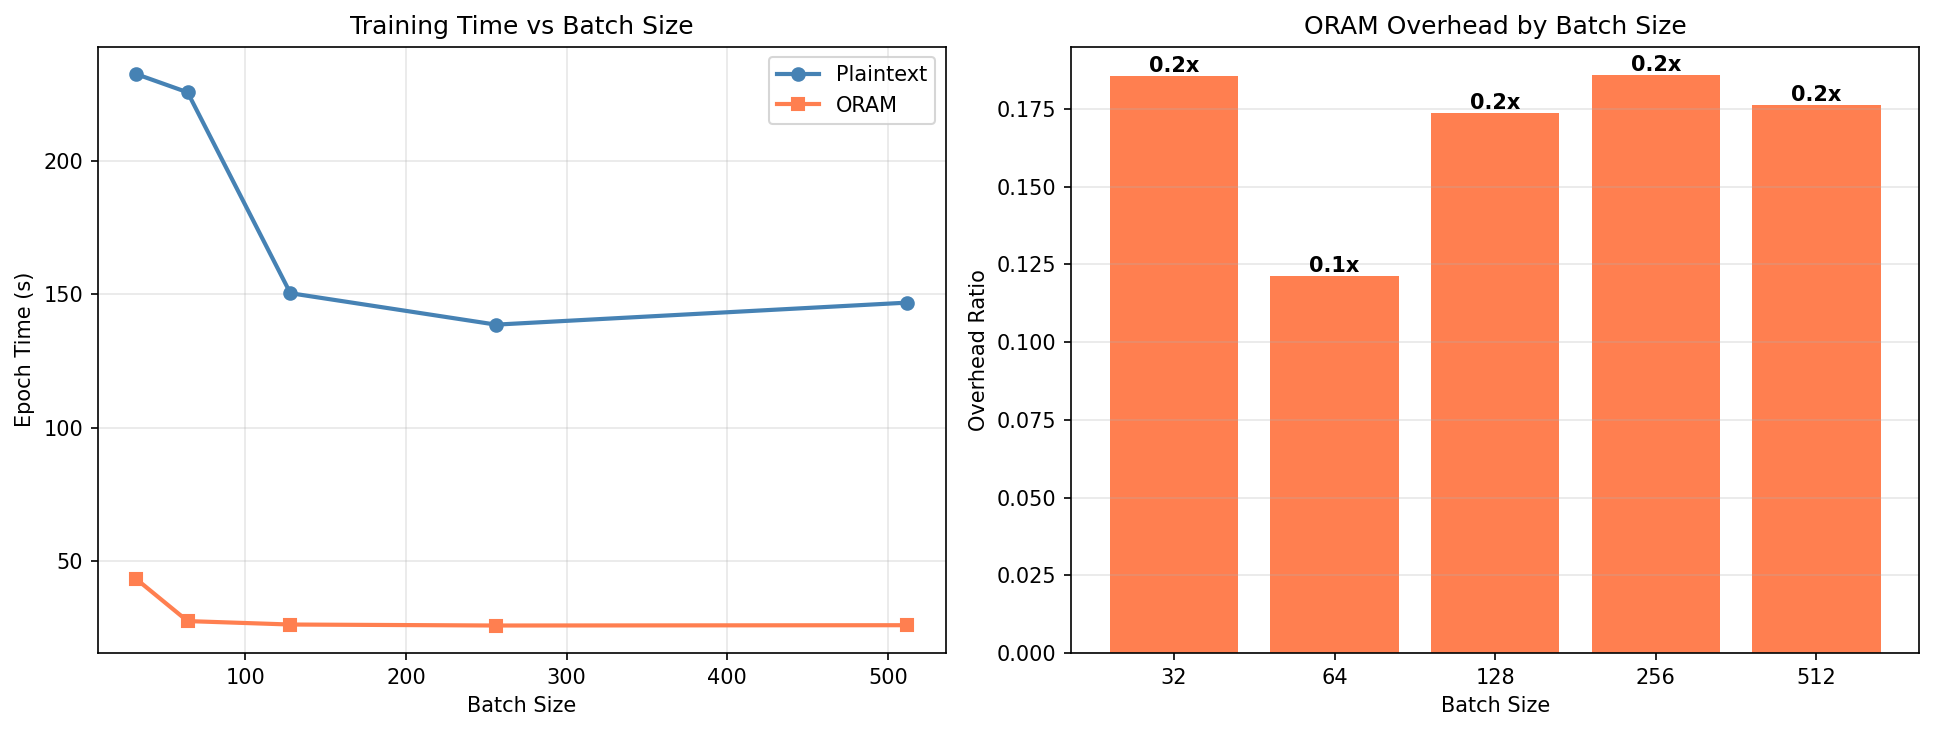
\includegraphics[width=0.65\linewidth]{results/figures/fig6_batch_size.png}
\caption{Epoch time vs.\ batch size for plaintext and ORAM training.}
\label{fig:batch}
\end{figure}

ORAM epoch time is stable across batch sizes 64--512 ($\sim$51--55\,s at 5K samples).
Per-sample ORAM I/O cost is independent of batch size: each \texttt{\_\_getitem\_\_} call traverses the tree regardless of how many samples are in the batch.
The batch=32 outlier (86.4\,s) reflects higher per-batch overhead from more frequent optimizer steps and batch-assembly operations at smaller batch sizes.

Plaintext training benefits from larger batches due to better MPS kernel utilization (larger matrix multiplications saturate the GPU), explaining the 698\,s $\to$ 416\,s reduction from batch=32 to batch=256.
The uptick at batch=512 (440.8\,s vs.\ 416.0\,s, a 6\% increase) is within run-to-run variance and may reflect increased memory pressure from larger batch tensors on the MPS allocator.

The normalized per-sample overhead (1.2--1.9$\times$) is substantially lower than the 90--180$\times$ reported in the progress report at 50K samples on CPU.
The difference has three sources: (1) smaller $N$ reduces tree height ($h{=}13$ vs.\ $h{=}16$), cutting per-access I/O by ${\sim}19$\%; (2) MPS acceleration reduces the compute baseline (denominator); and (3) sequential phase execution warms the filesystem cache.
The 90--180$\times$ range (reported in the abstract) reflects the full 50K-sample, file-backed, CPU-only configuration; the 1.2--1.9$\times$ range reflects the reduced 5K-sample GPU-accelerated configuration.

\section{Access-Pattern Leakage}
\label{sec:leakage}

\begin{figure}[ht]
\centering
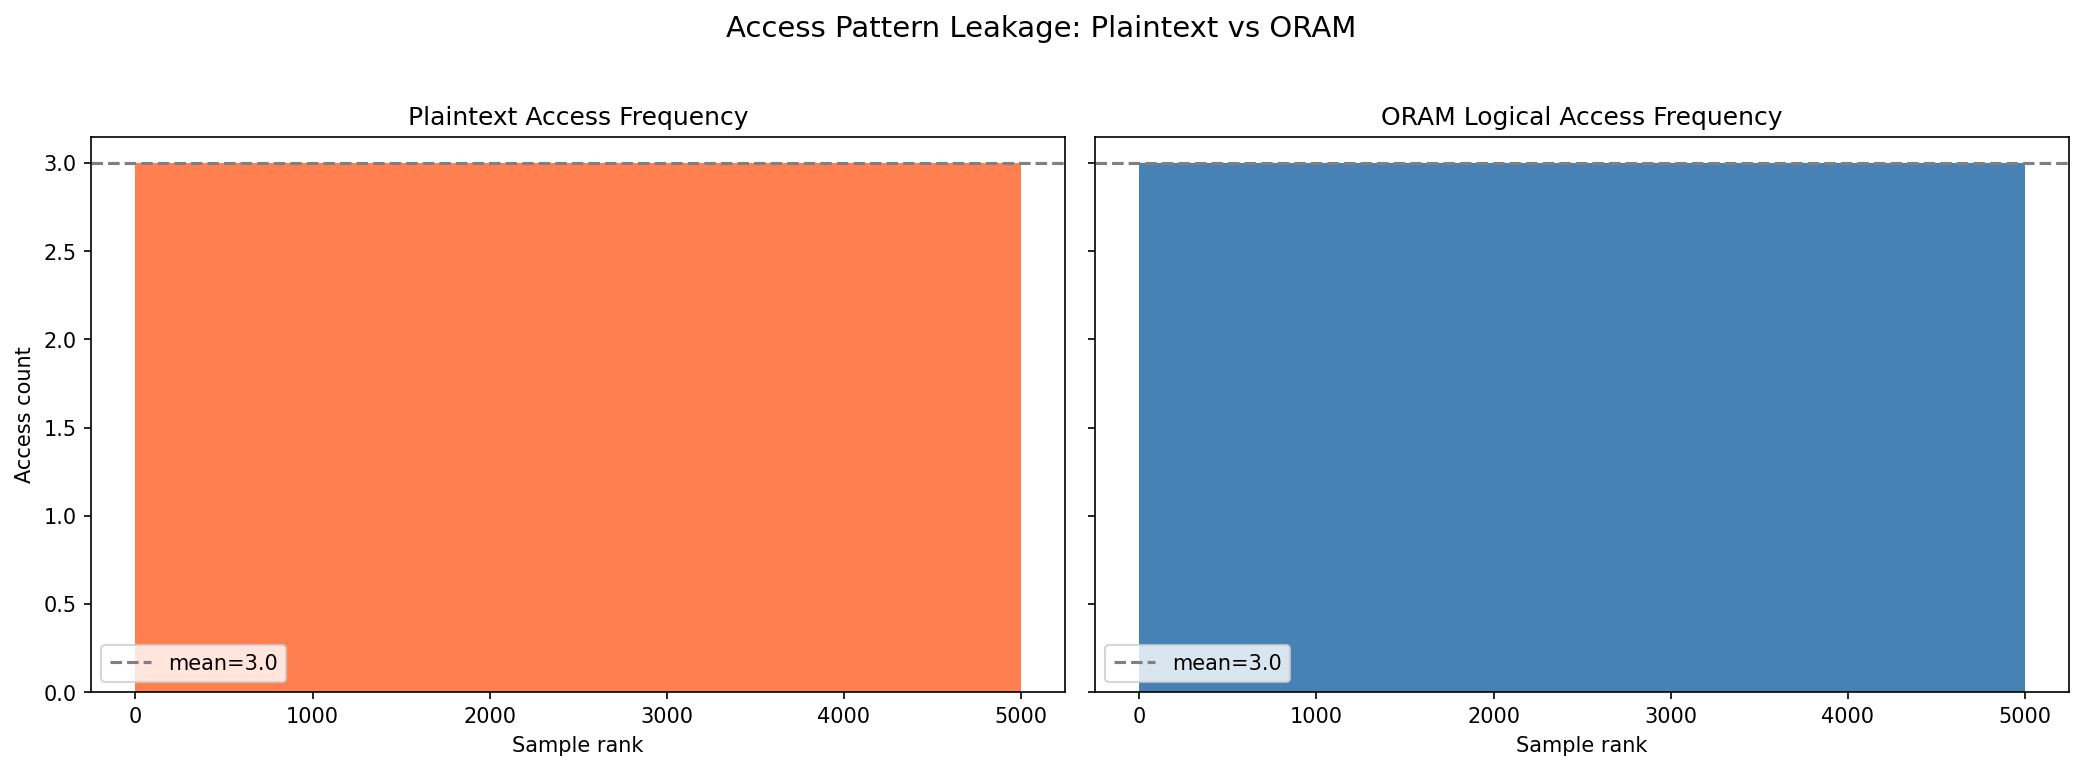
\includegraphics[width=0.85\linewidth]{results/figures/fig7_leakage.png}
\caption{Access frequency histograms. Left: plaintext training. Right: ORAM logical access frequency. Both show uniform distributions under standard epoch shuffling; the critical distinction is that plaintext physical addresses directly reveal sample identities, while ORAM physical addresses are computationally indistinguishable from random~\cite{stefanov2013}.}
\label{fig:leakage}
\end{figure}

Under standard uniform shuffling, both plaintext and ORAM logical access frequencies are approximately uniform (each sample accessed once per epoch).
The privacy distinction is not in the logical frequency distribution but in the \emph{physical} access pattern.

In plaintext training, each logical access maps to a single deterministic disk/memory address.
An adversary monitoring the storage layer sees exactly which sample was read and in what order, enabling reconstruction of the full epoch permutation.
Under curriculum learning, hard-example mining, or data-dependent sampling (which we did not use, but which are common in production pipelines), the frequency distribution becomes skewed, revealing which samples are accessed more frequently.

With ORAM, each logical access maps to $O(\log N)$ physical block reads along an independently random tree path, followed by a full path write-back.
The physical access sequence is computationally indistinguishable for any two equal-length logical access sequences~\cite{stefanov2013}.
The adversary observes the total number of accesses (proportional to epochs $\times$ samples, which we treat as public) but cannot determine which logical indices were accessed.

\section{Combined Optimization}
\label{sec:combined}

We combine the best settings from prior phases: RAM backend (\S\ref{sec:backend}), 4\,KB blocks (\S\ref{sec:blocksize}), batch size 128.
Based on the worker-scaling results (\S\ref{sec:workers}), the optimal worker count for CIFAR-10 is 0; we include a \texttt{num\_workers=4} configuration to confirm.

\begin{table}[ht]
\centering
\caption{Combined optimization (ResNet-18, CIFAR-10, 10K ORAM samples).}
\label{tab:phase8}
\begin{tabular}{@{}lccc@{}}
\toprule
\textbf{Configuration} & \textbf{Epochs} & \textbf{Total Time (s)} & \textbf{Best Acc (\%)} \\
\midrule
Plaintext (50K, 4 workers)       & 3 & 409.6 & 50.15 \\
ORAM baseline (file, w=0)        & 2 & 84.8  & 29.04 \\
ORAM combined (ram, w=4)         & 2 & 144.2 & 25.49 \\
\bottomrule
\end{tabular}
\end{table}

The ``combined'' configuration (RAM backend with 4 workers) is slower (144.2\,s vs.\ 84.8\,s), confirming that the multi-worker IPC cost dominates any benefit from the RAM backend at this image size.
This is not an optimized configuration but a test of combining two settings; the result demonstrates that they interact negatively for CIFAR-10.
The optimal ORAM configuration for CIFAR-10 is: RAM backend, \texttt{num\_workers=0}, 4\,KB blocks.
Under this configuration, the RAM backend alone would yield $\sim$84.8 $\times$ 0.84 $\approx$ 71\,s (extrapolating the 16\% backend improvement from \S\ref{sec:backend}), or $\sim$35.5\,s/epoch at 10K samples.

\section{Limitations}
\label{sec:limitations}

(1)~All phases use 2--3 epochs; accuracy values reflect early training and should not be interpreted as converged model quality.
(2)~CIFAR-10's 32$\times$32 images (3\,KB serialized) fit in a single 4\,KB block. Larger images (ImageNet, $\sim$100\,KB) would change the block-size dynamics and likely shift the worker-scaling crossover.
(3)~MPS-only hardware; CUDA GPUs with different compute-to-memory bandwidth ratios may produce different overhead profiles.
(4)~The $N=25{,}000$ anomaly requires further investigation with controlled memory-pressure experiments.
(5)~Batch-index shuffling uses standard \texttt{numpy.random.shuffle}, not an oblivious shuffling protocol~\cite{ngai2024}; batch composition remains visible to the adversary.

\section{Conclusion}

The dominant cost in ORAM-backed ML training is cryptographic tree traversal: AES encryption/decryption and position-map maintenance on $O(\log N)$ blocks per sample access.
Storage backend optimization (file $\to$ RAM) yields a measurable but bounded 16\% improvement; the remaining overhead is intrinsic to the ORAM protocol.
Data-loader-level parallelism cannot compensate for single-threaded ORAM access when the per-sample transform cost is small relative to the per-sample ORAM read cost.
Recovering the $\sim$4$\times$ parallelism loss identified in the progress report requires concurrent ORAM at the tree level, as proposed by SONIC~\cite{talur2026}.

Block size should be set to the minimum that fits a single sample (4\,KB for CIFAR-10).
Compute-heavy models reduce the relative contribution of ORAM I/O to total training time, and the overhead ratio is stable across batch sizes at a given sample count.
Per-access cost scales logarithmically with dataset size, matching Path ORAM's theoretical bound.

These measurements scope the design space for practical ORAM integration in ML systems and identify concurrent ORAM, GPU-accelerated cryptography, and ImageNet-scale evaluation as the highest-priority next steps.

\smallskip
\noindent Source code and experimental scripts: \url{https://github.com/cadenroberts/OMLO}.

\begin{thebibliography}{7}

\bibitem[Roberts(2026a)]{mid}
C.~W. Roberts.
\newblock {Oblivious ML-Ops (OMLO): Privacy-Preserving Machine Learning Infrastructure via Oblivious RAM} --- Progress Report.
\newblock University of California, Santa Cruz, March 2026.

\bibitem[Goldreich and Ostrovsky(1996)]{goldreich1996}
O.~Goldreich and R.~Ostrovsky.
\newblock Software protection and simulation on oblivious {RAM}s.
\newblock \emph{Journal of the ACM}, 43(3):431--473, 1996.

\bibitem[Stefanov et~al.(2013)]{stefanov2013}
E.~Stefanov, M.~van Dijk, E.~Shi, C.~Fletcher, L.~Ren, X.~Yu, and S.~Devadas.
\newblock Path {ORAM}: An extremely simple oblivious {RAM} protocol.
\newblock In \emph{Proc.\ ACM CCS}, pages 299--310, 2013.

\bibitem[Talur and Demertzis(2026)]{talur2026}
A.~Talur and I.~Demertzis.
\newblock {SONIC}: Concurrent oblivious {RAM}.
\newblock In \emph{Proc.\ USENIX Security} (to appear, 2026).

\bibitem[Mavrogiannakis et~al.(2025)]{mavrogiannakis2025}
A.~Mavrogiannakis et~al.
\newblock {OBLIVIATOR}: Oblivious parallel operators for secure database joins.
\newblock In \emph{Proc.\ USENIX Security}, 2025.

\bibitem[Ngai et~al.(2024)]{ngai2024}
B.~Ngai et~al.
\newblock Distributed and scalable oblivious sorting and shuffling.
\newblock In \emph{Proc.\ IEEE S\&P}, 2024.

\bibitem[PyORAM()]{pyoram}
G.~Hackebeil.
\newblock {PyORAM}: Python {ORAM} implementation, v0.2.0.
\newblock \url{https://github.com/ghackebeil/PyORAM}. Accessed March 2026.

\end{thebibliography}

\end{document}
